\section{Toric Code II}
\subsection{Review}
A quick review of some definitions; the Toric code has Hamiltonian (defined on a 2D lattice with qubits placed on the edges):
\begin{equation}
    H = - \sum_s A_s - \sum_p B_p
\end{equation}
with $A_s$ star operators around each lattice vertex:
\begin{equation}
    A_s = \prod_{j \in \text{star}(s)}X_s
\end{equation}
and $B_p$ plaquette operators around each lattice plaquette
\begin{equation}
    B_p = \prod_{j \in \partial p}Z_p
\end{equation}
we constructed the ground state $\ket{\Omega} = \ket{a_s = b_p = 1}$. We also discussed a string operator, which creates charge excitations:
\begin{equation}
    W^Z(\gamma) = \prod_{j \in \gamma}Z_j
\end{equation}
where $\gamma$ is a path on the lattice. It creates charges ($a_s = -1$) at the endpoints of $\gamma$. Further, these string operators are flexible, in the sense that:
\begin{equation}
    W^Z(\gamma)\ket{\Omega} = W^Z(\gamma')\ket{\Omega}
\end{equation}
for two paths $\gamma, \gamma'$ with the same endpoints.

\subsection{String operator for flux excitations}
There is a similar string operator for flux excitations. Just a heads up that the structure of having string operators (one for each anyon type - here for charges and fluxes/$e$ and $m$) is quite general. We define:
\begin{equation}
    W^X(\hat{\gamma}) = \prod_{j \in \hat{\gamma}}X_j
\end{equation}
where $\hat{\gamma}$ is an open path on the dual lattice, i.e. that go through the center of plaquettes:

\begin{center}
    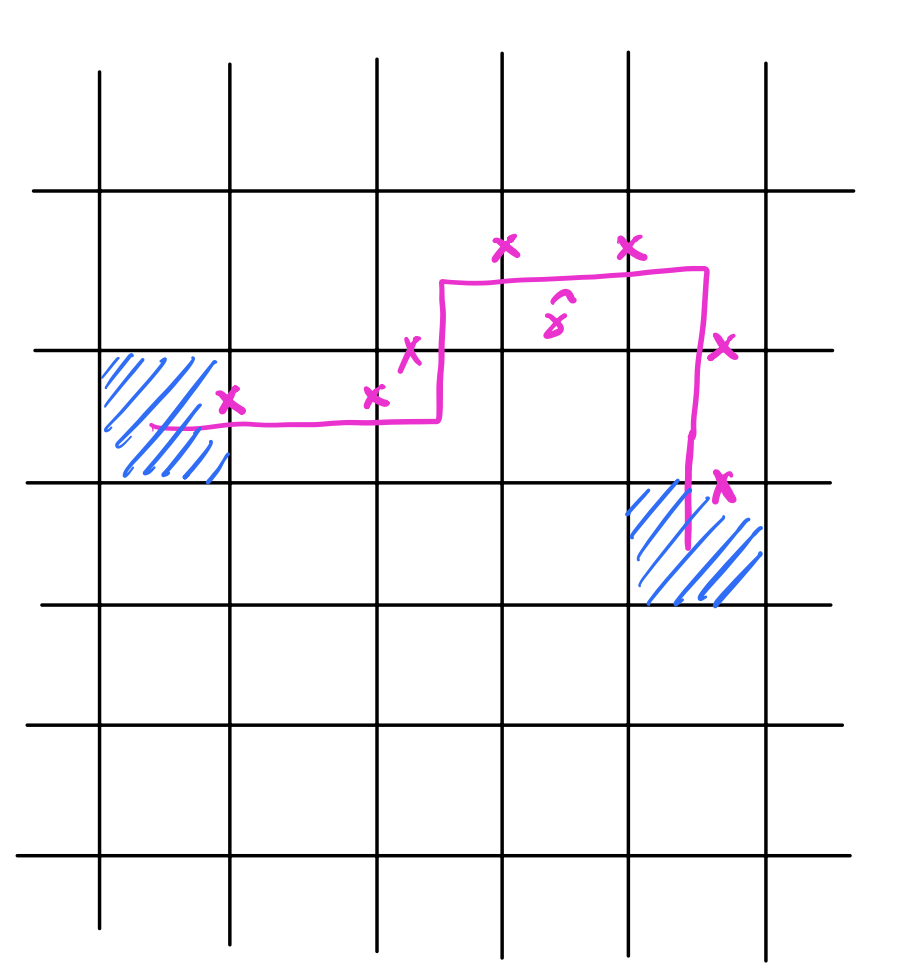
\includegraphics[scale=0.4]{Lectures/Images/lec2-fluxstring.png}
\end{center}

Much like the string operator for the charges:
\begin{itemize}
    \item It can be checked that $W^X(\hat{\gamma})$ creates fluxes $b_p = -1$ at the two endpoints of $\hat{\gamma}$.
    \item The string operators are flexible, with:
    \begin{equation}
        W^X(\hat{\gamma})\ket{\Omega} = W^X(\hat{\gamma}')\ket{\Omega}
    \end{equation}
    for $\hat{\gamma}, \hat{\gamma}'$ with the same endpoints. They are related by the product of star operators on the interior.
    \begin{center}
        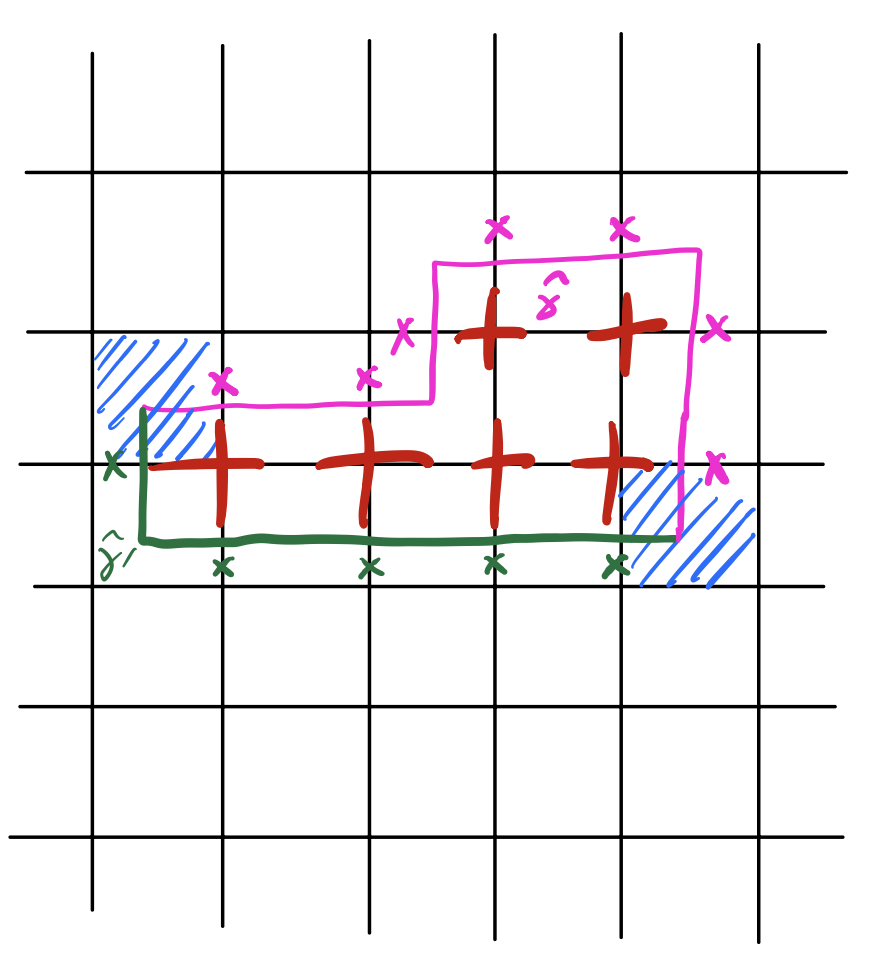
\includegraphics[scale=0.4]{Lectures/Images/lec2-fluxstring2.png}
    \end{center}
\end{itemize}

The existence of these flexible, non-commuting string operators is very fundamental to the structure of the toric code, and to anyon systems more generally. The existence of these is independent of geometries. But we will see that it will have implications when we consider the model for specific systems.

\subsection{Ground state degeneracy on a torus}
\begin{center}
    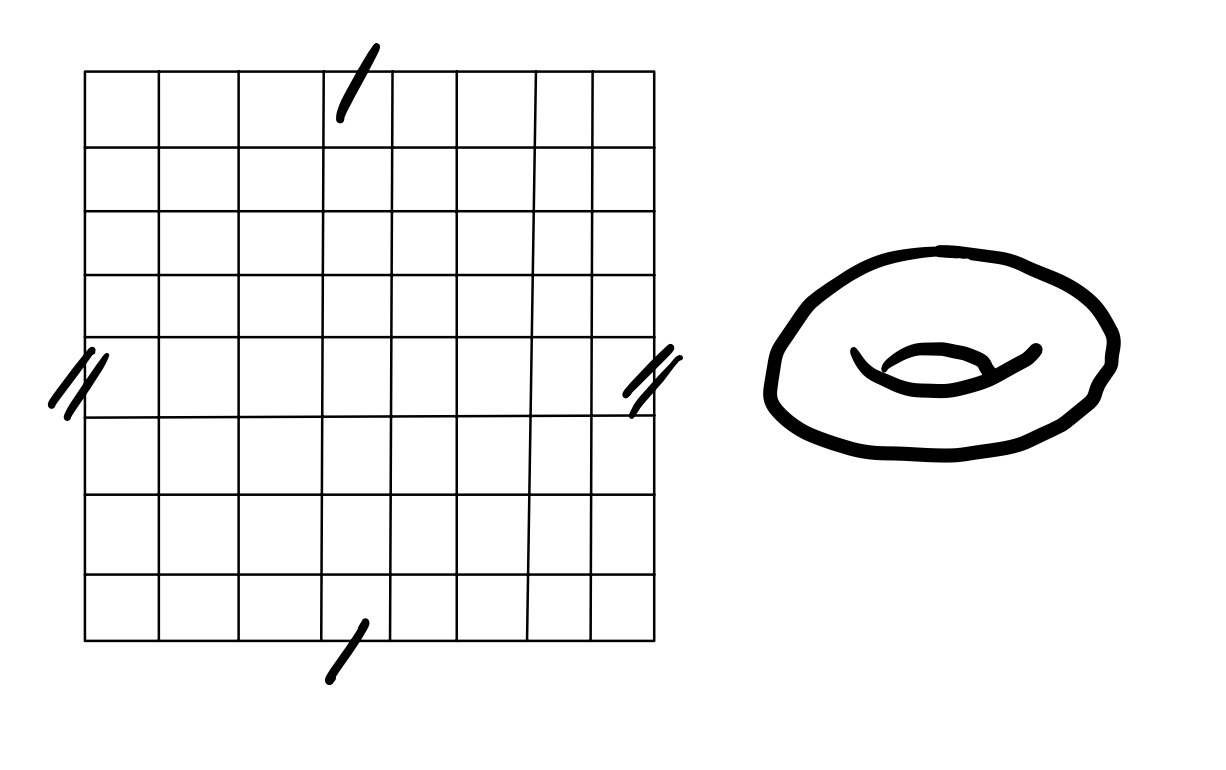
\includegraphics[scale=0.4]{Lectures/Images/lec2-torus.png}
\end{center}
Consider the toric code, on a finite ($L \times L$) torus. We may have different allowable states for a given $a_s$ and $b_p$, and thus may find that there are different degeneracies, compared to the infinite plane case.  We can now ask what is the ground state degeneracy $D$? Indeed, this question is equivalent to asking what the dimension of the eigenspace with $a_s = b_p = 1$ is. To find this, we look at the trace of the projector onto the eigenspace\footnote{This is a very formal way to find it, we will soon get different perspectives on this question}:
\begin{equation}
    \begin{split}
        D &= \Tr(\text{proj. onto $a_s = b_p = 1$ subspace})
        \\ &= \Tr(\prod_{s}\left(\frac{\II + A_s}{2}\right)\prod_{p}\left(\frac{\II + B_p}{2}\right))
    \end{split}
\end{equation}
where the second line follows from the fact that the product of the (mutually commuting) projectors gives the projector onto the subspace. Computing this:
\begin{equation}
    D = \frac{1}{2^{N_s}}\frac{1}{2^{N_p}}\Tr(\prod_{s}(\II + A_s)\prod_{p}(\II + B_p))
\end{equation}
Now we expand out this product, and can think about the traces of the individual terms. A single $A_s, B_p$ will be traceless (as the Paulis are traceless), and so will most products of $A_s, B_p$; the only non-traceless terms will be those that simplify to the identity. If we stare at this, there are only a few combinations for which this occurs; there is the term with all identity, the term with all stars (all the $X$s cancel), the term with all plaquettes (all the $Z$s cancel), and the term with all stars and all plaquettes.
\begin{equation}
    D = \frac{1}{2^{N_s}}\frac{1}{2^{N_p}}\Tr(\II + \prod_s A_s + \prod_p B_p + \prod_s\prod_p A_sB_p) = \frac{1}{2^{N_s}}\frac{1}{2^{N_p}}\Tr(4\II)
\end{equation}
Now looking at the trace of the identity:
\begin{equation}
    \Tr(\II) = 2^{\text{dim}(\mathcal{H})} = 2^{N_{\text{links}}}
\end{equation}
Thus:
\begin{equation}
    D = \frac{1}{2^{L^2}}\cdot \frac{1}{2^{L^2}} \cdot 4 \cdot 2^{2L^2} = 4
\end{equation}
so:
\begin{equation}
    \boxed{D = 4}
\end{equation}
A nice feature of this argument is we can repeat it for any of the eigenspaces. In fact, every $\set{a_s, b_p}$ eigenspace with $\prod_s a_s = \prod_p b_p = 1$ (i.e. an even number of charges) is 4-fold degenerate. 

\subsection{Ground states in the string picture}

Now, let's see if we can understand the ground state degeneracy in the string picture. To review, we work in the $X$-basis, and $X_j = \pm 1$ corresponds to there being a string (plus) or no string on link $j$. $a_s = 1$ requires the product of $X$s on the star to be one, implying that the strings form closed loops. $b_p = 1$  implies that there is an equal amplitude superposition of string states, as different string states are related by $B_p$ moves. We used these two conditions on the infinite plane geometry (Where $B_p$ moves are ``ergodic'') to say that there was a unique ground state, namely that with an equal weight superposition of all closed loop configurations:
\begin{equation}
    \ket{\Omega} = \sum_{\text{closed loop config $C$}}\ket{C}
\end{equation}
On a torus, the closed loop states can be divided into 4 classes; even/even, even/odd, odd/even, and odd/odd. 

\begin{center}
    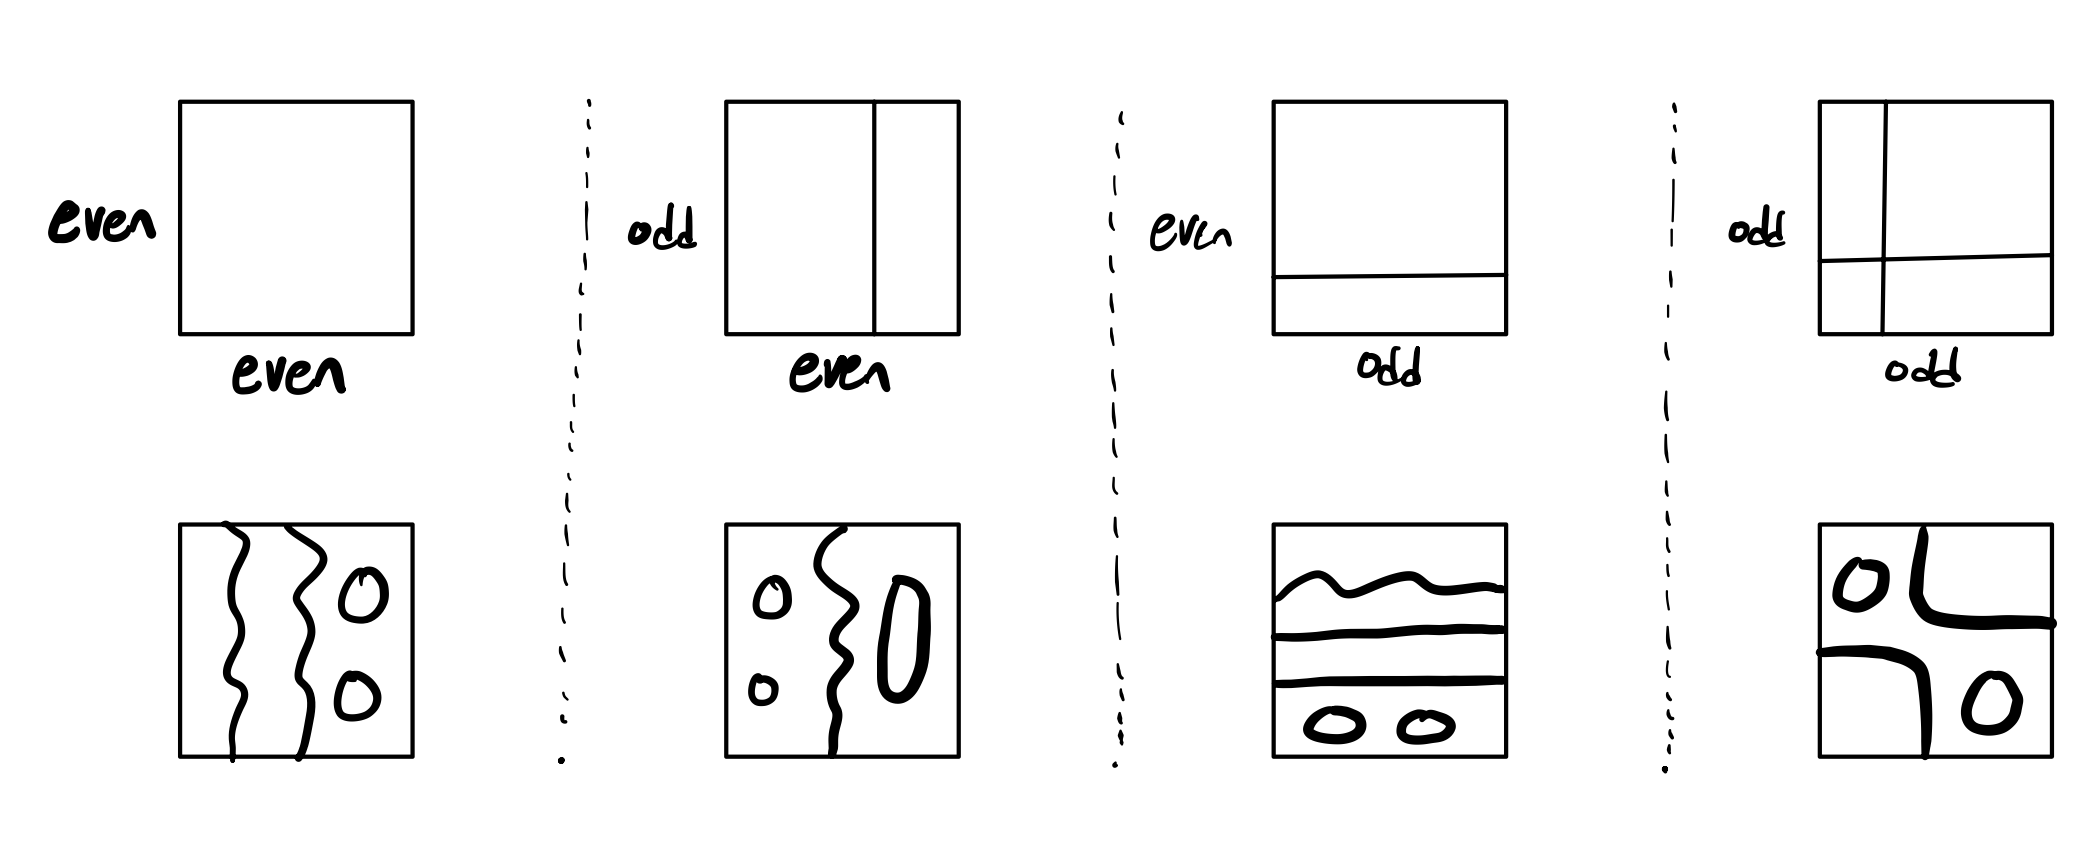
\includegraphics[scale=0.4]{Lectures/Images/lec2-evenodd.png}
\end{center}

What does this mean? this means that if we draw a line going across the torus (on the dual lattice), we ``cross'' an even/odd number of strings. Within each sector/class, the $B_p$ moves are ergodic. But, $B_p$ moves cannot change the parity of the crossings. Thus the four degenerate ground states correspond to the equal weight superpositions of closed loop configurations within a given class. We can label the ground states via their winding number:
\begin{equation}
    \ket{\Omega_{(e/o, e/o)}} = \sum_{\text{closed loop config $C$ with (e/o, e/o) winding}}\ket{C}
\end{equation}

So, so far we have understood the ground state degeneracy from two perspectives. But neither of these tells us the deeper principle underlying the degeneracy. Let us discuss this now - it will allow us to see why the degeneracy is topologically protected.

\subsection{Origin of the ground state degeneracy}
The punchline is that the GSD comes from the existence of non-commuting string operators.

Define the charge string operators:
\begin{equation}
    W_1^Z = \prod_{j \in \gamma_1}Z_j
\end{equation}
\begin{equation}
    W_2^Z = \prod_{j \in \gamma_2}Z_j
\end{equation}
These string operators correspond to the creation and subsequent annihilation of a charge as the string wraps around the torus. We can also define the string operators for the fluxes;
\begin{equation}
    W_1^X = \prod_{j \in \hat{\gamma}_1}X_j
\end{equation}
\begin{equation}
    W_2^X = \prod_{j \in \hat{\gamma}_2}X_j
\end{equation}

\begin{center}
    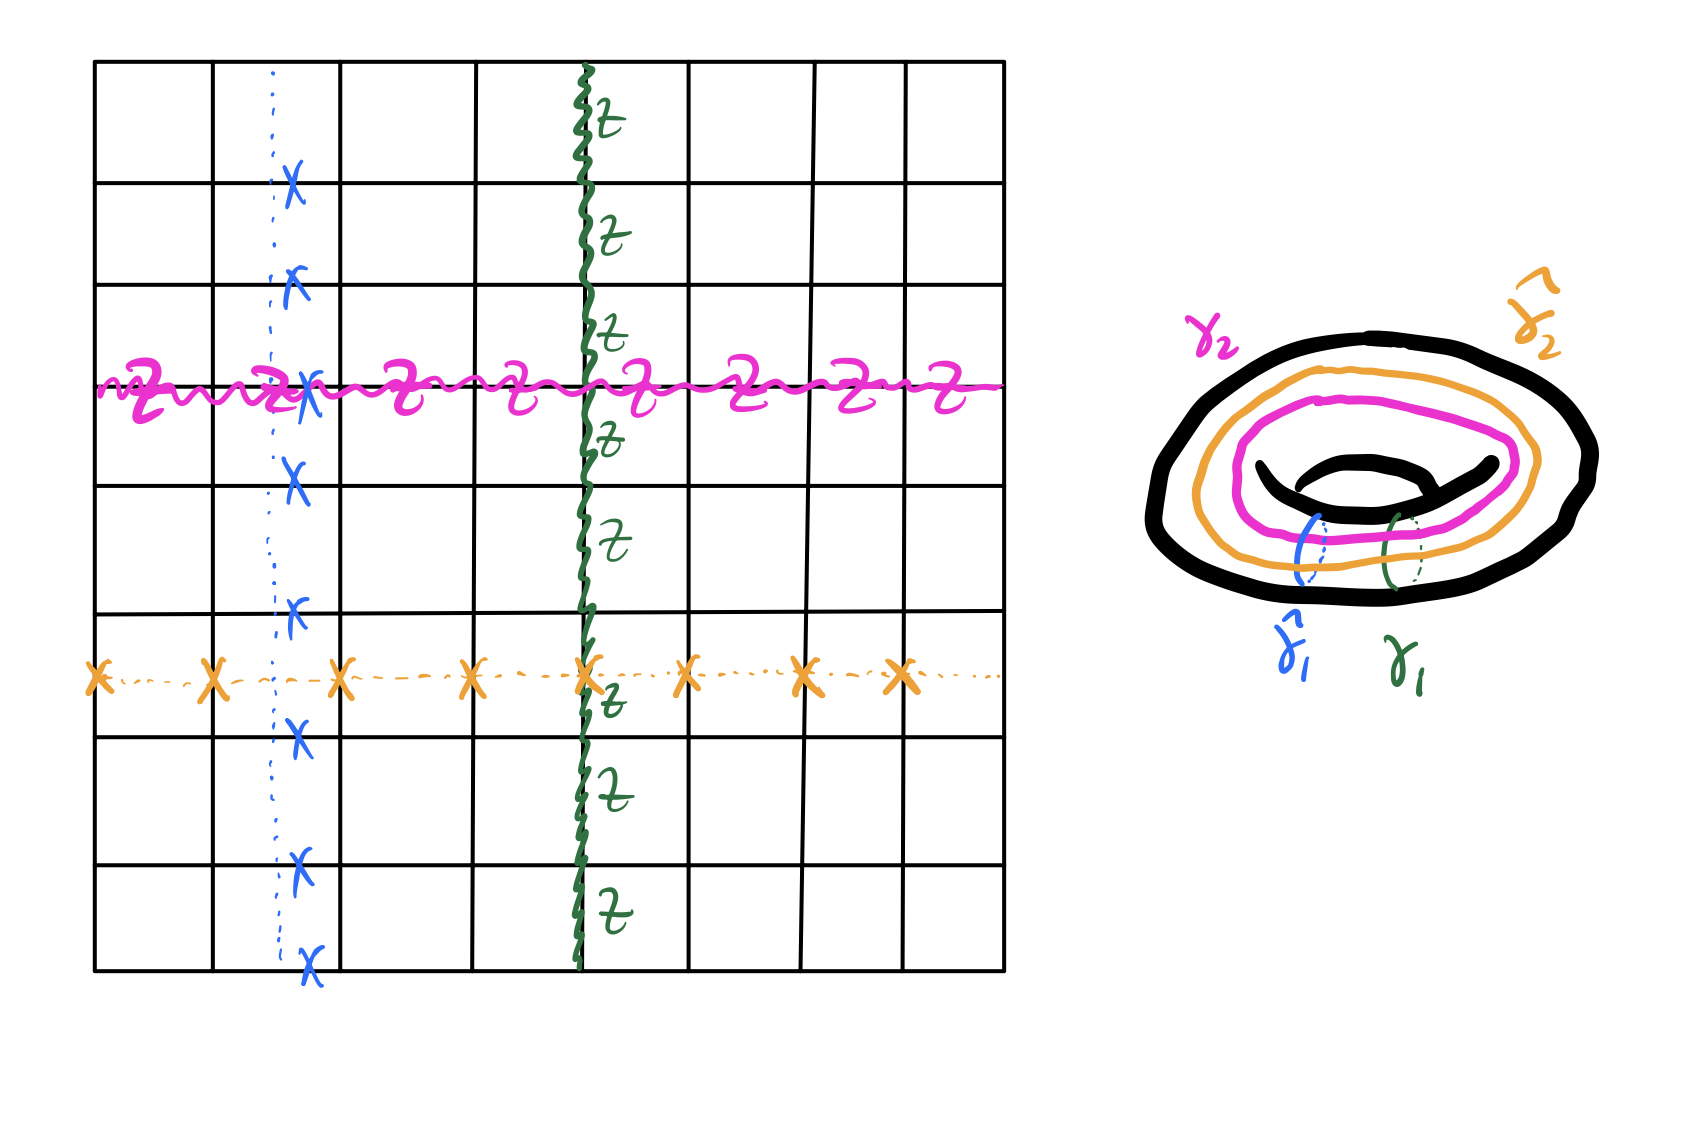
\includegraphics[scale=0.4]{Lectures/Images/lec2-torusstrings.png}
\end{center}

Notice that:
\begin{equation}
    \begin{split}
        [W_i^Z, A_s] &= [W_i^Z, B_p] = 0
        \\ [W_i^X, A_s] &= [W_i^X, B_p] = 0
    \end{split}
\end{equation}
so they map ground states to ground states. They have an interesting commutation algebra. $\set{W_1^Z, W_2^Z, W_1^X, W_2^X}$ all commute, except for two exceptions:
\begin{equation}
    \begin{split}
        W_1^XW_2^Z &=  -W_2^ZW_1^X
        \\ W_2^XW_1^Z &=  -W_1^ZW_2^X
    \end{split}
\end{equation}
this is because they anticommute in one place.

\begin{center}
    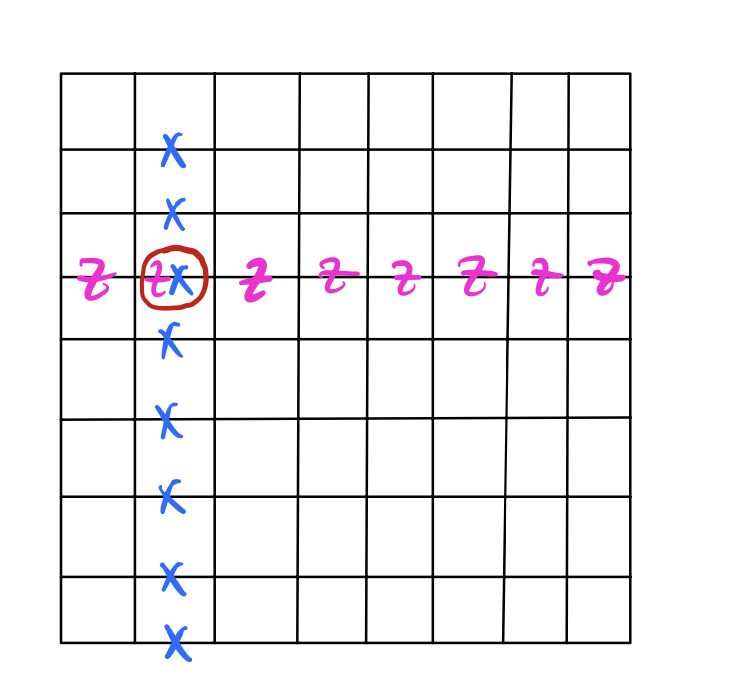
\includegraphics[scale=0.4]{Lectures/Images/lec2-torusanticommute.png}
\end{center}

The fact that the other commute is clear; the fact that the $X$s mutually commute and $Z$s mutually commute is immediate. For $W_1^X, W_1^Z$, they act on disjoint regions. Even if you were to pick representatives that overlap, they will overlap an even amount of times.

\begin{center}
    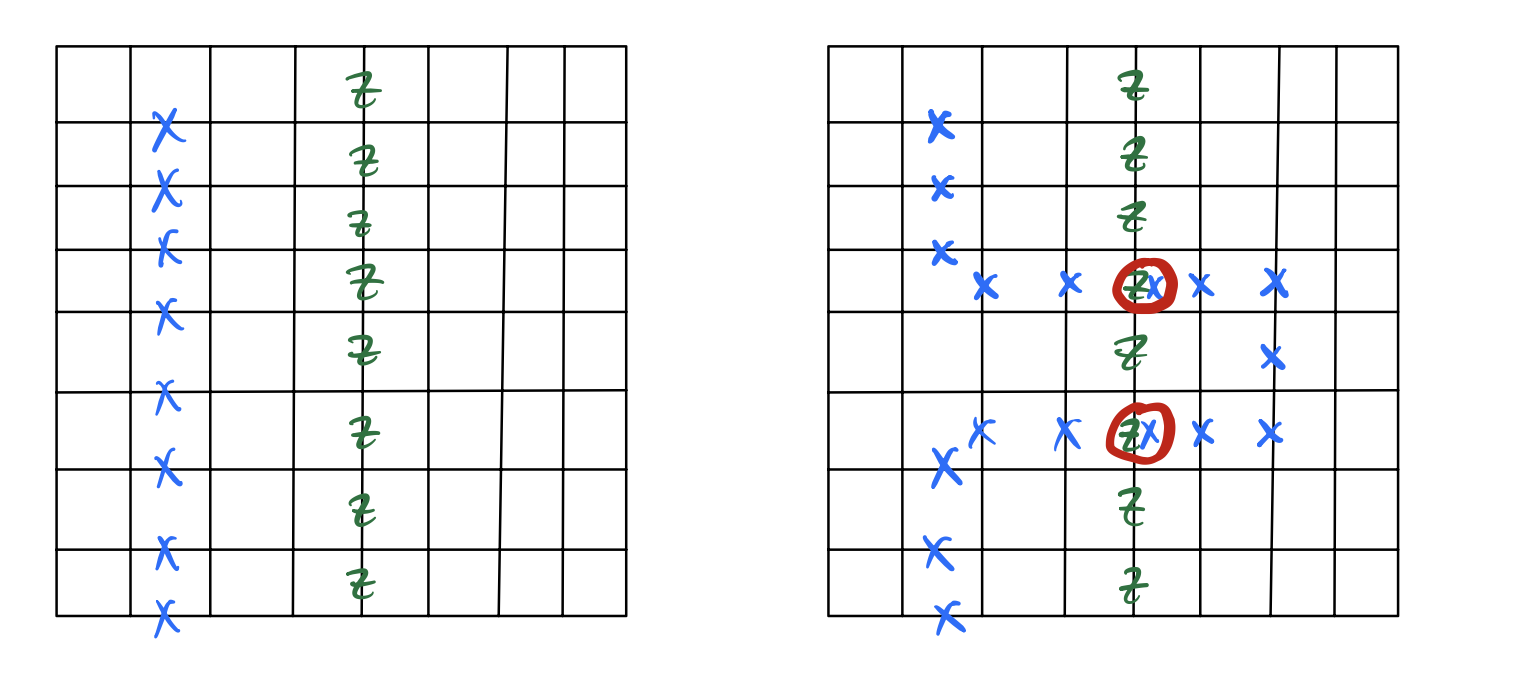
\includegraphics[scale=0.4]{Lectures/Images/lec2-toruscommute.png}
\end{center}

This algebra is quite interesting; we have symmetry generators that commute with the Hamiltonian, but not with each other. A simple HW exercise you will do is that the eigenstates/ground states will come in multiplets of 4 (the fact that it is exactly 4 in this case comes from the microscopic calculation).

A final comment; we said how the $\set{a_s, b_p}$ do not uniquely specify the ground (or excited) states. But in fact the string operators provide the missing quantum numbers necessary to specify the state. Specifically, we can uniquely label the eigenstates by choosing (in addition to the $\set{a_s, b_p}$) the values of the $W$s, e.g $\ket{\set{a_s, b_p}, w_1^x, w_2^x}$ where $w_1^x = \pm 1$ and $w_2^x = \pm 1$. We can thus denote the four ground states as $\ket{\Omega, \pm\pm}$. These are \emph{exactly} the same what we called before the $\ket{\Omega_{(e/o, e/o)}}$ - in fact the $W^x$ string operator counts the number of crossing of $X$ strings.

Next time, we will discuss how the GSD is robust to arbitrary local perturbations - it is topologically protected.